\documentclass[frenchb]{article}
\usepackage[T1]{fontenc}
\usepackage[latin1]{inputenc}
%Pour utilisation sous unix
%\usepackage[utf8]{inputenc}
%\usepackage[utf8x]{inputenc}
\usepackage{a4wide}
\usepackage{graphicx}
\usepackage{amssymb}
\usepackage{color}
\usepackage{babel}
\usepackage{tabto}

\begin{document}

\begin{figure}[t]
\centering

\includegraphics[width=5cm]{inp_n7.png}
\end{figure}

\title{\vspace{4cm} \textbf{Manuel d'utilisation}}
\author{Issam Alouane\\Jean-Baptiste Prevost\\\\�quipe GH11 }	
\date{\vspace{7cm} D�partement Sciences du Num�rique - Premi�re ann�e \\
2021-2022 }

\maketitle

\newpage
\tableofcontents
\listoffigures
\newpage
\section{Mise en place}

Avant de pouvoir utiliser la compression et la d�compression il est n�cessaire de pr�parer un environnement dans lequel les faire fonctionner.\\

Pour cela veuillez ouvrir une console comme le montre la figure \ref{fig : console} ci-dessous:\\
\begin{figure}[ht!]
    \centering
    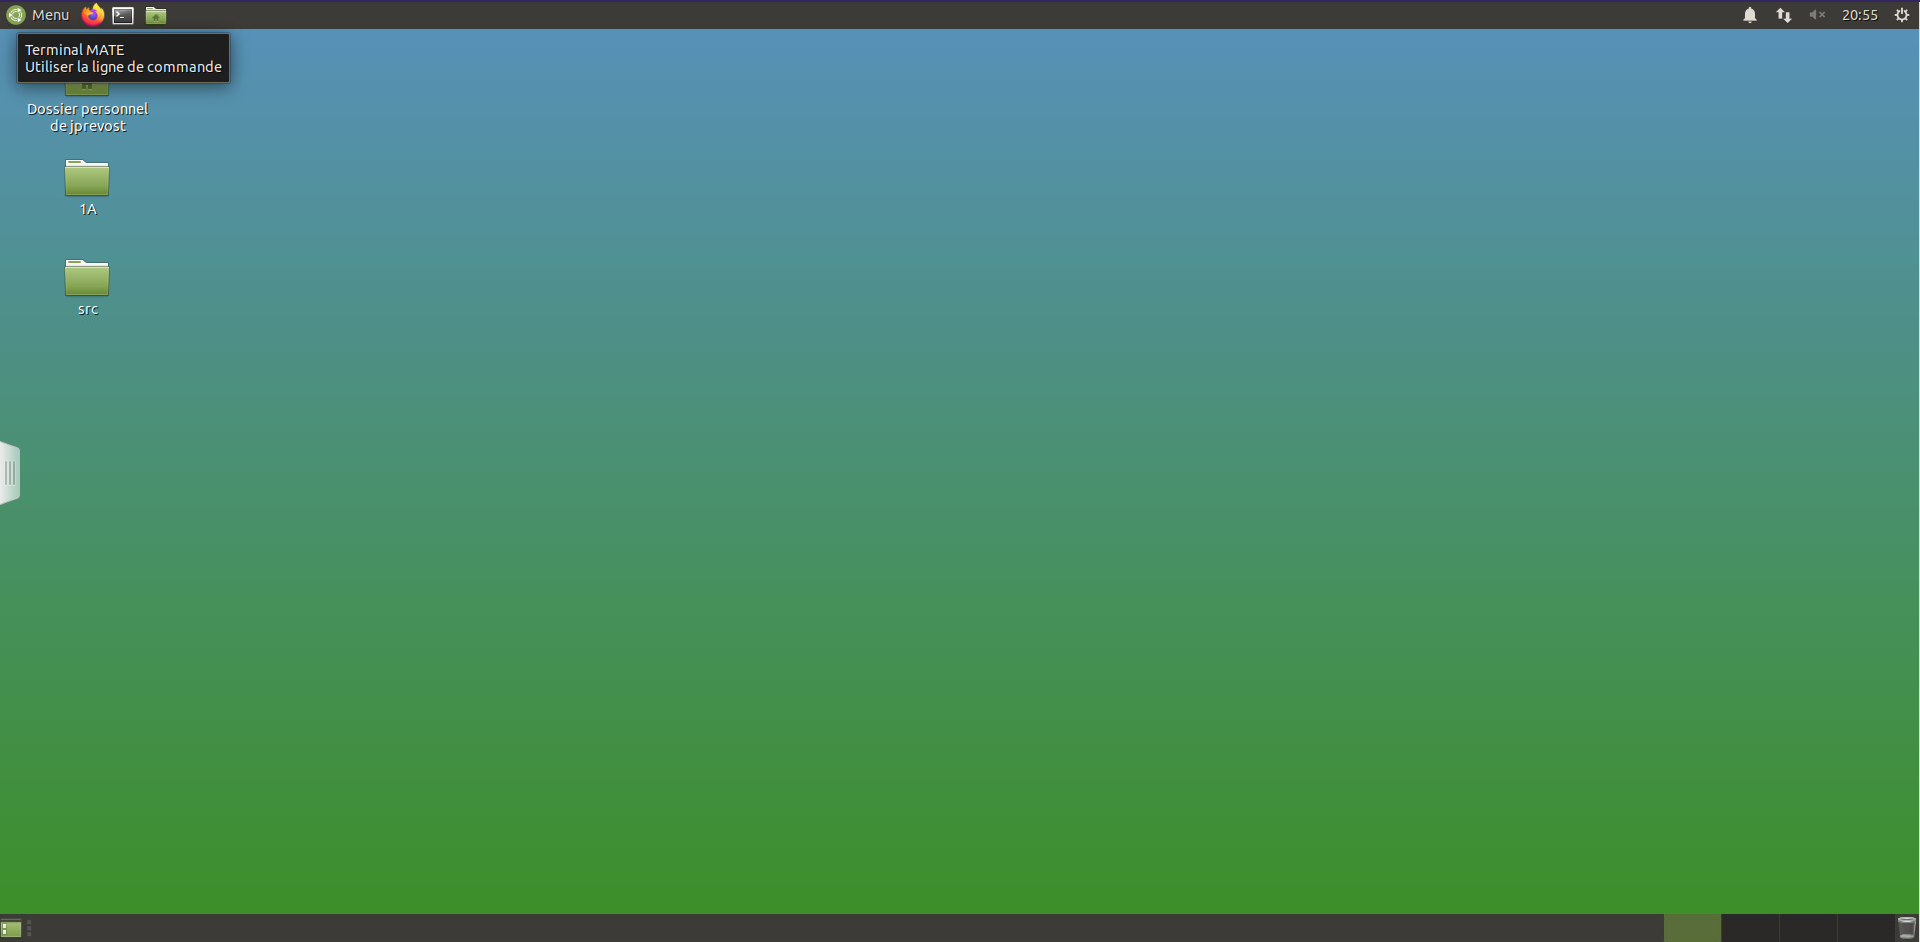
\includegraphics[width=15cm]{console.png}
    \caption{Ouverture de l'environnement d'ex�cution \label{fig : console}}
\end{figure}
 
Maintenant que votre espace de travail est initialis� vous devez vous rendre dans le r�pertoire des ex�cutables comme le montre la figure \ref{fig : r�pertoire}.
 
\begin{figure}[ht!]
    \centering
    \includegraphics[width=15cm]{repertoire.png}
    \caption{R�pertoire des ex�cutables \label{fig : r�pertoire}}
\end{figure}

Vous voila maintenant pr�t a utiliser les ex�cutables de compression et de d�compression.

\section{Utilisation Compression}

Il existe plusieurs mode de fonctionnement pour le programme de compression. Dans un premier temps nous allons utiliser le mode muet de celui-ci. Pour cela il faut appeler l'ex�cutable puis mettre en argument un seul fichier a compresser, comme le montre la figure \ref{fig : compression}.\\

\begin{figure}[ht!]
    \centering
    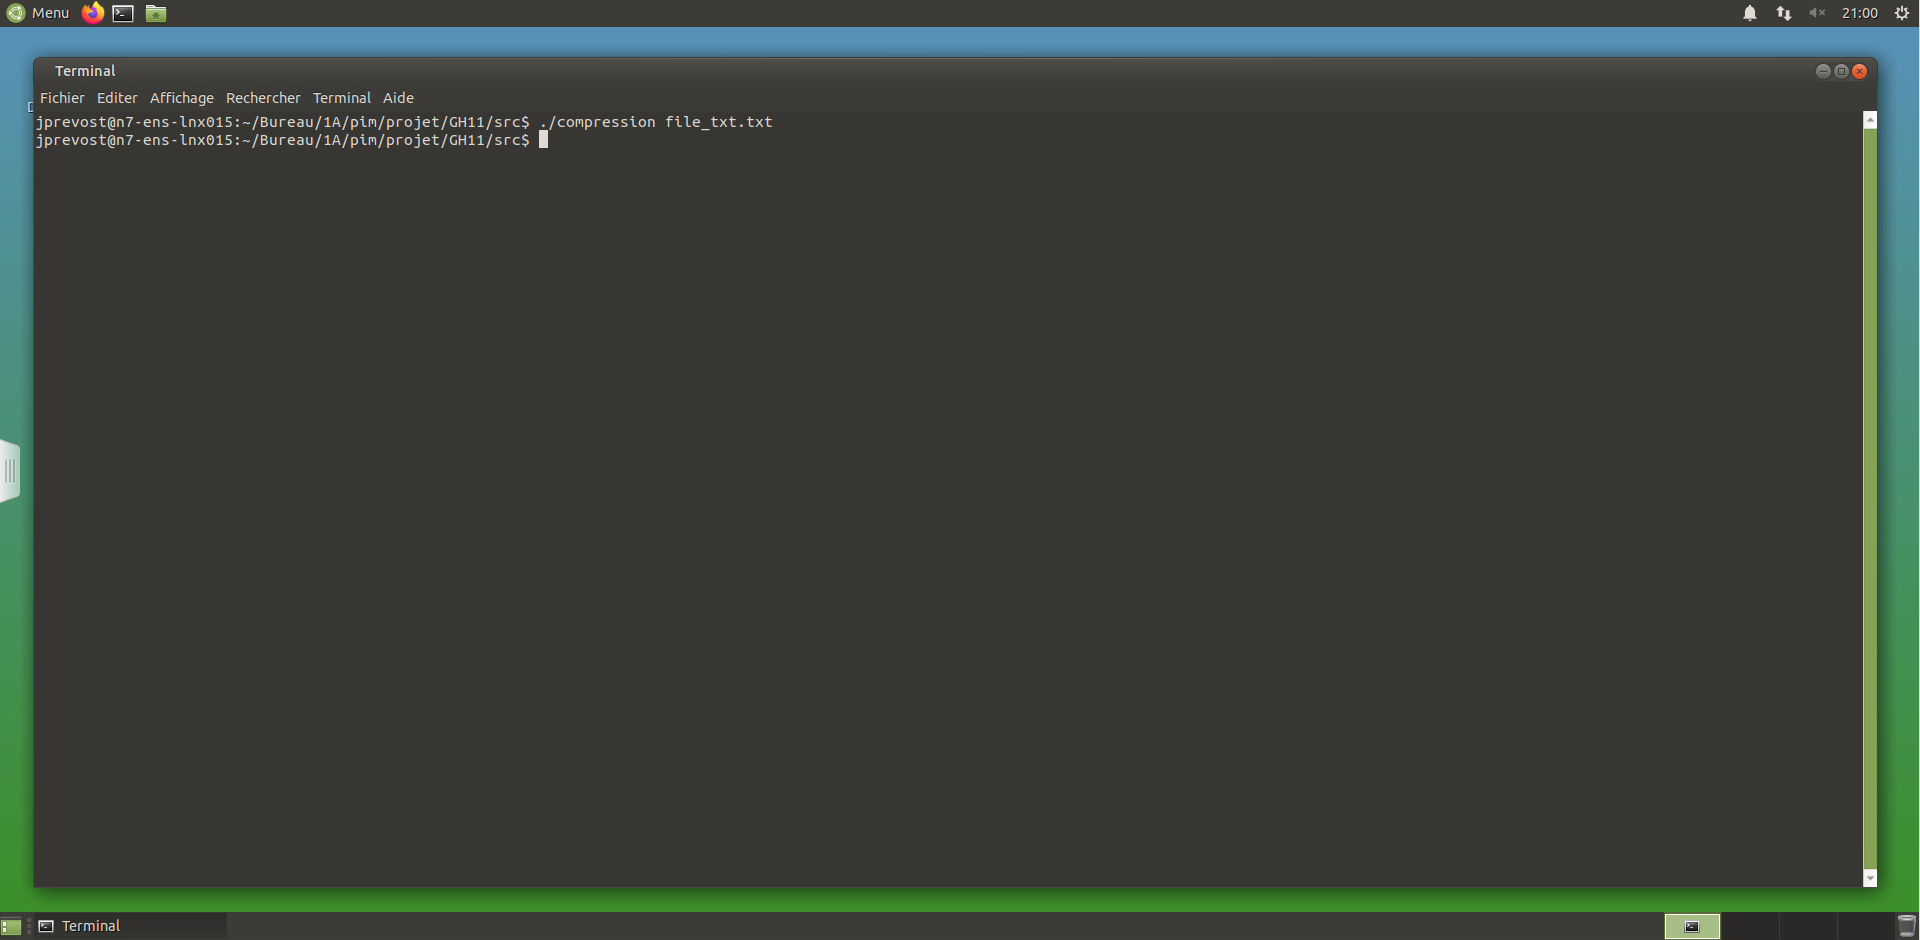
\includegraphics[width=15cm]{compression.png}
    \caption{Compression muette \label{fig : compression}}
\end{figure}

Pour ex�cuter le mode bavard de ce programme il suffit de mettre en premier argument $-b$ ou $--bavard$ suivi du fichier � compresser. Vous devriez obtenir un r�sultat similaire � la figure \ref{fig : compression_b}\\

\begin{figure}[ht!]
    \centering
    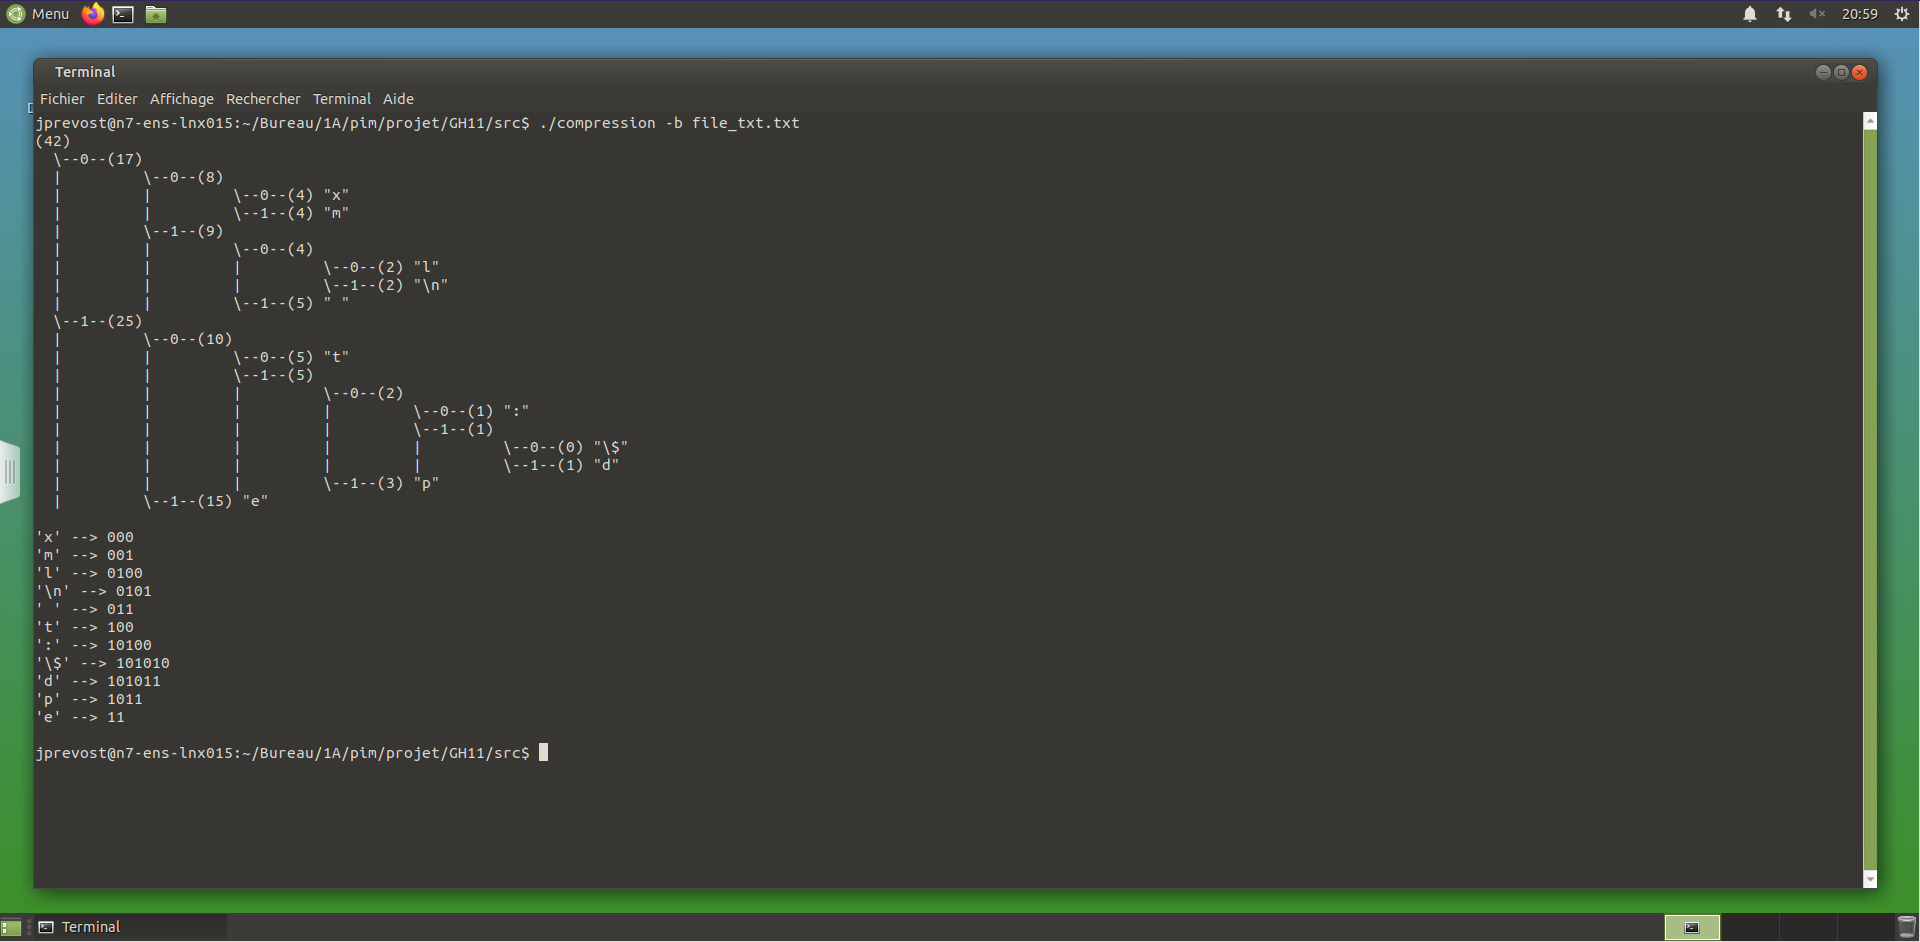
\includegraphics[width=15cm]{compression_b.png}
    \caption{Compression bavarde \label{fig : compression_b}}
\end{figure}

On retrouve bien l'arbre d'Huffman ainsi que sa table associ�e.

\section{Utilisation D�compression}

Maintenant que le fichier est compress� il serait utile de pouvoir le d�compresser pour cela il suffit d'appeler le programme de d�compression et de mettre en argument le fichier a d�compresser. Attention tout de fois, a v�rifier que le fichier � d�compresser soit d'extension $.hff$\\

\begin{figure}[ht!]
    \centering
    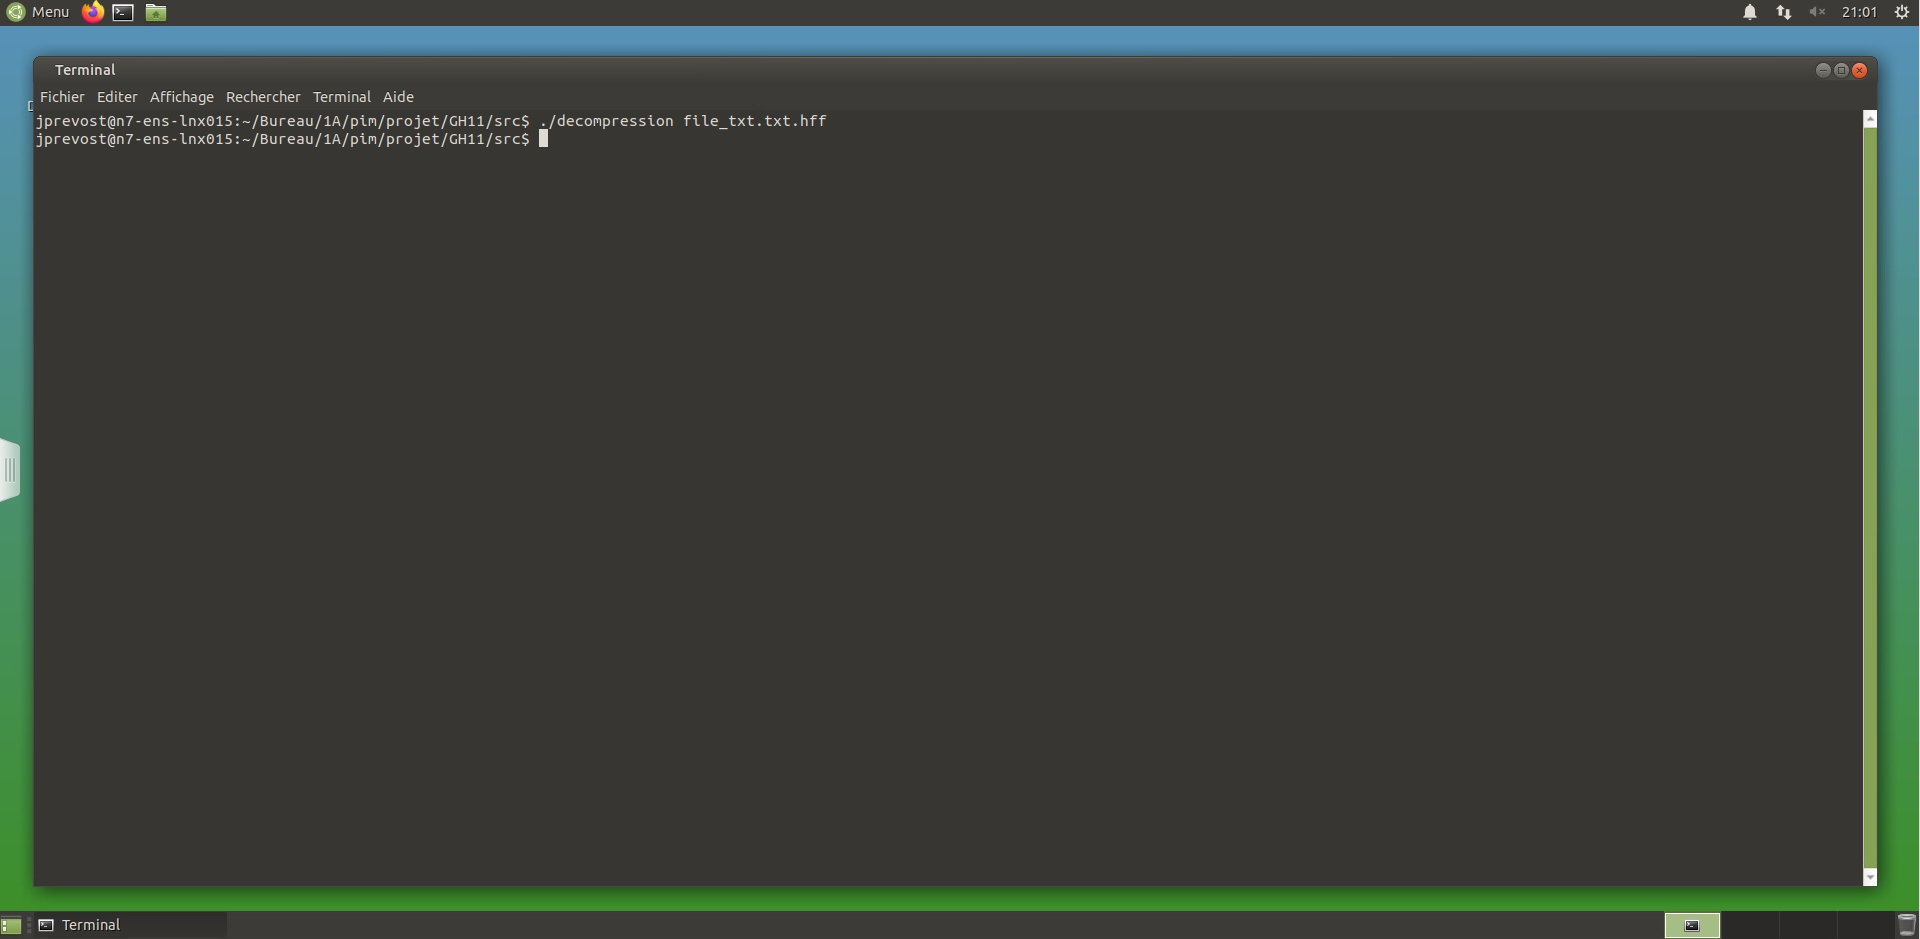
\includegraphics[width=15cm]{decompression.png}
    \caption{D�compression \label{fig : decompression}}
\end{figure}

Vous devez maintenant pouvoir acc�der au fichier d�compress�.

\end{document} 